\chapter{API Module Inventory}
\label{app:modules}

Table~\ref{tab:modules-full} lists NestJS modules registered in \texttt{app.module.ts}.

\begin{longtable}{@{}p{3.2cm}p{10.8cm}@{}}
  \caption{NestJS feature modules in MedPrepAI backend.} \label{tab:modules-full} \\
  \toprule
  \textbf{Module} & \textbf{Responsibility} \\
  \midrule
  \endfirsthead
  \multicolumn{2}{c}{\tablename\ \thetable\ -- \textit{Continued}} \\
  \toprule
  \textbf{Module} & \textbf{Responsibility} \\
  \midrule
  \endhead
  Auth, Users, Roles & Authentication, profiles, RBAC \\
  Products, Categories, Systems & Catalog and taxonomies \\
  Content, Questions & Hierarchy and QBank CRUD \\
  Assessments, MockExams & Papers, timed exams \\
  Subscriptions, Payments & Billing, Stripe, entitlements \\
  MedprepAi & Clinical encounter sessions \\
  AiTutor & Tutoring conversations \\
  Faculty, Institution & Assignments, cohorts \\
  Chat, Notifications, Realtime & Messaging \\
  Bookmarks, Notes, Flashcards & Study tools \\
  StudyPlans, Goals, StudentStats & Planning and analytics \\
  Achievements & Badges and points \\
  Discussions, StudyGroups & Community \\
  Feedback, QuestionReports & Support \\
  \bottomrule
\end{longtable}

\chapter{MedPrep Database Tables}
\label{app:medprep-tables}

\begin{table}[htbp]
  \centering
  \caption{MedPrep-related database tables.}
  \label{tab:medprep-tables}
  \begin{tabular}{@{}lp{9.5cm}@{}}
    \toprule
    \textbf{Table} & \textbf{Purpose} \\
    \midrule
    medprep\_conversations & Session header: mode, status, score \\
    medprep\_conversation\_messages & Chat transcript \\
    medprep\_diagnosis\_submissions & Learner vs.\ actual diagnosis \\
    medprep\_soap\_notes & SOAP + AI feedback \\
    medprep\_hint\_sessions & Learning mode hint usage \\
    \bottomrule
  \end{tabular}
\end{table}

\chapter{Frontend Route Map}
\label{app:routes}

\begin{longtable}{@{}p{4.5cm}p{9.5cm}@{}}
  \caption{Selected Next.js pages.} \label{tab:routes} \\
  \toprule
  \textbf{Route} & \textbf{Purpose} \\
  \midrule
  \endfirsthead
  \toprule
  \textbf{Route} & \textbf{Purpose} \\
  \midrule
  \endhead
  /landing-page & Marketing, pricing, FAQ \\
  /practice-mode & MedPrep Practice \\
  /learning-mode & MedPrep Learning \\
  /evaluation & MedPrep Evaluation \\
  /shadow-mode & MedPrep Shadow \\
  /dashboard & Student home \\
  /faculty, /faculty/compare & Faculty workspace \\
  /test-creation/* & Build question papers \\
  /test-session/[id] & Timed test \\
  /payments/* & Billing UI \\
  /messages, /chat/rooms & Messaging \\
  /assignments & Institution assignments \\
  /soap/[conversationId] & SOAP editor \\
  /admin & Administration \\
  \bottomrule
\end{longtable}

\chapter{Environment Variables}
\label{app:env}

\begin{table}[htbp]
  \centering
  \caption{Core environment variables.}
  \label{tab:env-vars}
  \small
  \begin{tabular}{@{}lp{8.5cm}@{}}
    \toprule
    \textbf{Variable} & \textbf{Purpose} \\
    \midrule
    DATABASE\_URL & MySQL connection string \\
    JWT\_SECRET & Token signing \\
    GOOGLE\_API\_KEY / GEMINI\_API\_KEY & Gemini LLM \\
    GEMINI\_MODEL & Model id (default 2.5 Flash) \\
    STRIPE\_SECRET\_KEY & Payments \\
    NEXT\_PUBLIC\_API\_URL & Frontend $\rightarrow$ backend \\
    \bottomrule
  \end{tabular}
\end{table}

\chapter{Demo Seed and Reproducibility}
\label{app:seed}

\begin{verbatim}
cd backend
npm run prisma:seed:demo
# Reset demo data:
./scripts/seed-demo-full.sh --reset
\end{verbatim}

Demo entities are prefixed \texttt{[Demo]} for easy identification in UI and database queries.

\chapter{Development Timeline}
\label{app:timeline}

Figure~\ref{fig:gantt} summarizes major implementation phases described in Chapter~1.

\begin{figure}[htbp]
  \centering
  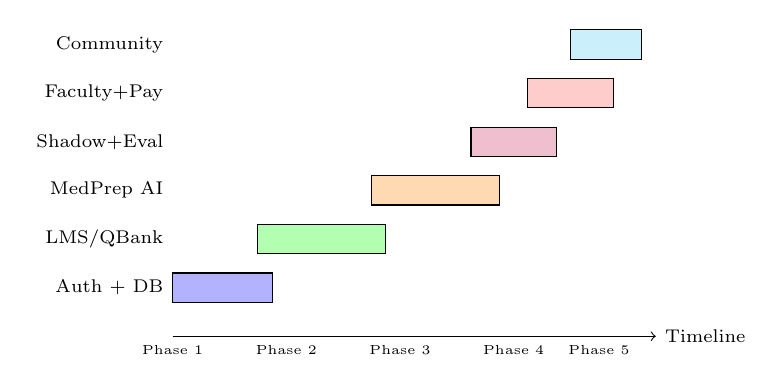
\begin{tikzpicture}[x=0.38cm, y=0.65cm, scale=0.95, transform shape]
    \draw[->] (0,0) -- (17,0) node[right,font=\scriptsize]{Timeline};
    \foreach \x/\m in {0/Phase 1, 4/Phase 2, 8/Phase 3, 12/Phase 4, 15/Phase 5} {
      \node[font=\tiny, below] at (\x,0) {\m};
    }
    \node[left, font=\scriptsize] at (0,1) {Auth + DB};
    \draw[fill=blue!30] (0,0.7) rectangle (3.5,1.3);
    \node[left, font=\scriptsize] at (0,2) {LMS/QBank};
    \draw[fill=green!30] (3,1.7) rectangle (7.5,2.3);
    \node[left, font=\scriptsize] at (0,3) {MedPrep AI};
    \draw[fill=orange!30] (7,2.7) rectangle (11.5,3.3);
    \node[left, font=\scriptsize] at (0,4) {Shadow+Eval};
    \draw[fill=purple!25] (10.5,3.7) rectangle (13.5,4.3);
    \node[left, font=\scriptsize] at (0,5) {Faculty+Pay};
    \draw[fill=red!20] (12.5,4.7) rectangle (15.5,5.3);
    \node[left, font=\scriptsize] at (0,6) {Community};
    \draw[fill=cyan!20] (14,5.7) rectangle (16.5,6.3);
  \end{tikzpicture}
  \caption{Project development timeline (approximate phases).}
  \label{fig:gantt}
\end{figure}


\chapter{Stakeholder Analysis}
\label{app:stakeholders}

\begin{table}[htbp]
  \centering
  \caption{Stakeholders and platform value proposition.}
  \label{tab:stakeholders}
  \small
  \begin{tabular}{@{}p{2.8cm}p{5.5cm}p{5.7cm}@{}}
    \toprule
    \textbf{Stakeholder} & \textbf{Needs} & \textbf{MedPrepAI response} \\
    \midrule
    Medical student & Practice encounters, QBank, feedback & Four modes + assessments \\
    Faculty & Monitor cohort, assign cases & Faculty workspace \\
    Institution & License software, branding & Subscriptions + domains \\
    Administrator & Content, users, billing & Admin + payments \\
    Developer & Extensible APIs & Nest modules + Swagger \\
    \bottomrule
  \end{tabular}
\end{table}

\chapter{Glossary}
\label{app:glossary}

\begin{table}[htbp]
  \centering
  \caption{Glossary of terms.}
  \begin{tabular}{@{}lp{9.5cm}@{}}
    \toprule
    \textbf{Term} & \textbf{Definition} \\
    \midrule
    OSCE & Objective Structured Clinical Examination \\
    SOAP & Subjective, Objective, Assessment, Plan documentation \\
    QBank & Question bank for exam preparation \\
    VP & Virtual patient \\
    RBAC & Role-based access control \\
    LLM & Large language model \\
    LMS & Learning management system \\
    DDx & Differential diagnosis \\
    JWT & JSON Web Token \\
    \bottomrule
  \end{tabular}
\end{table}
